\chapter{Planificación y costes}\label{planificacion}

En esta sección repasaremos la planificación detallada del proyecto, esto incluye una lista completa de actividades así como un desglose de horas.

\section{Listado completo de actividades}

\renewcommand{\arraystretch}{1.5}
\begin{longtable}{|p{0.03\linewidth}|p{0.52\linewidth}|p{0.105\linewidth}|p{0.1\linewidth}|p{0.1\linewidth}|}

    % cabecera
    \hline \textbf{Id} & \textbf{Descripción} & \textbf{Ámbito} & \textbf{Prioridad}  & \textbf{Horas}\\ \hline \endhead
    
    % memoria
    1 & Lectura y comprensión del artículo principal & Memoria & Crítica & 7.5 \\ \hline
    2 & Consulta de artículos matemáticos de soporte para aclarar y completar ideas & Memoria & Crítica & 15 \\ \hline
    3 & Consulta de artículos relacionados con SIKE de soporte para aclarar y completar ideas & Memoria & Crítica & 5 \\ \hline
    4 & Desarrollo de un índice primitivo & Memoria & Alto & 0.5 \\ \hline
    5 & Redacción de las secciones matemáticas de la memoria & Memoria & Medio & 45 \\ \hline
    6 & Redacción de las secciones criptográficas de la memoria & Memoria & Medio & 45 \\ \hline
    7 & Redacción de las secciones técnicas de la memoria & Memoria & Medio & 45 \\ \hline
    8 & Correcciones y cambios tras revisiones propias y/o del tutor (incluye tutorías) & Memoria & Alto & 20 \\ \hline
    9 & Preparación de la presentación y estudio & Memoria & Alto & 3 \\ \hline

    % frontend
    10 & Idea general de la distribución de la interfaz & Frontend & Crítico & 0.5 \\ \hline
    11 & Vista de inicio & Frontend & Medio & 5 \\ \hline
    12 & Menú de protocolos & Frontend & Medio & 1.5 \\ \hline
    13 & Página de información & Frontend & Bajo & 1.5 \\ \hline
    14 & Vista de presentación de protocolo & Frontend & Crítico & 10 \\ \hline
    15 & Presentación del protocolo de prueba de identidad & Frontend & Bajo & 5 \\ \hline
    16 & Presentación del protocolo de intercambio de llave & Frontend & Alto & 15 \\ \hline
    17 & Presentación del protocolo de cifrado & Frontend & Alto & 20 \\ \hline
    18 & Conexión con el backend y contexto & Frontend & Alto & 7.5 \\ \hline
    19 & Correcciones de estilo en función del tamaño de la pantalla & Frontend & Bajo & 5 \\ \hline
    20 & Internacionalización de la interfaz & Frontend & Bajo & 5 \\ \hline
    21 & Diseñar e implementar el conjunto de pruebas & Frontend & Medio & 10 \\ \hline

    % backend
    22 & Diseño de la entidad base en función de las necesidades de la interfaz y el funcionamiento de la implementación de SIKE & Backend & Crítico & 0.5 \\ \hline
    23 & Implementar entidad y builder & Backend & Alto & 5 \\ \hline
    24 & Implementar capa de servicio & Backend & Alto & 1 \\ \hline
    25 & Implementar controladores & Backend & Alto & 1 \\ \hline
    26 & Modificar seguridad por defecto del proyecto Spring para el acceso a los endpoints & Backend & Alto & 5 \\ \hline
    27 & Diseñar e implementar el conjunto de pruebas & Backend & Medio & 10 \\ \hline

    % otros: soporte, despliegue, etc
    28 & Investigación y consulta para resolver problemas de implementación específicos & Soporte & Bajo & 25 \\ \hline
    29 & Investigación de medios y plataformas de despliegue disponibles & Despliegue & Alto & 5 \\ \hline
    30 & Despliegue y resolución de incidencias inmediatas relacionadas & Despliegue & Alto & 3 \\ \hline
    & TOTAL &&& 300 \\ \hline
    
    \caption{Listado completo de actividades y sus características}
    \label{tab:actividades}
\end{longtable}

\section{Cronograma}

En esta sección compararemos el trabajo planificado y lo compararemos con el trabajo real realizado.

\subsection{Estimación original}

En la figura \ref{fig:cronograma-original} tenemos la planificación original del proyecto. 


\subsection{Cronograma final y desviación}

En la figura \ref{fig:cronograma-real} tenemos el cronograma final del proyecto. 

La primera gran diferencia es la misma escala temporal, nuestra idea era presentarnos a la primera convocatoria. Una vez comenzamos a trabajar, vimos que la dedicación necesaria era mayor a la esperada y cada fase del proyecto se alargó. Las primeras fases, las de investigación y redacción de la memoria, son prácticamente idénticas si ignoramos la diferencias de fechas.

A la hora de la implementación gráfica si ha habido más desorden en comparación con la planificación original. El backend, que era lo primero que estaba previsto hacer, lo atrasamos hasta ya tener el frontend montado y la conexión con el frontend no lo hicimos una vez la aplicación estaba iniciada sino una vez realizamos el protocolo de cifrado.

El desarrollo del frontend siguió la planificación original (salvo a la hora de realizar cada uno de los protocolos, aunque este cambio no es relevante realmente) en mayor parte porque esta planificación seguía el orden lógico de interacción con la página.


\begin{landscape}
\begin{figure}[!ht]
    \centering
    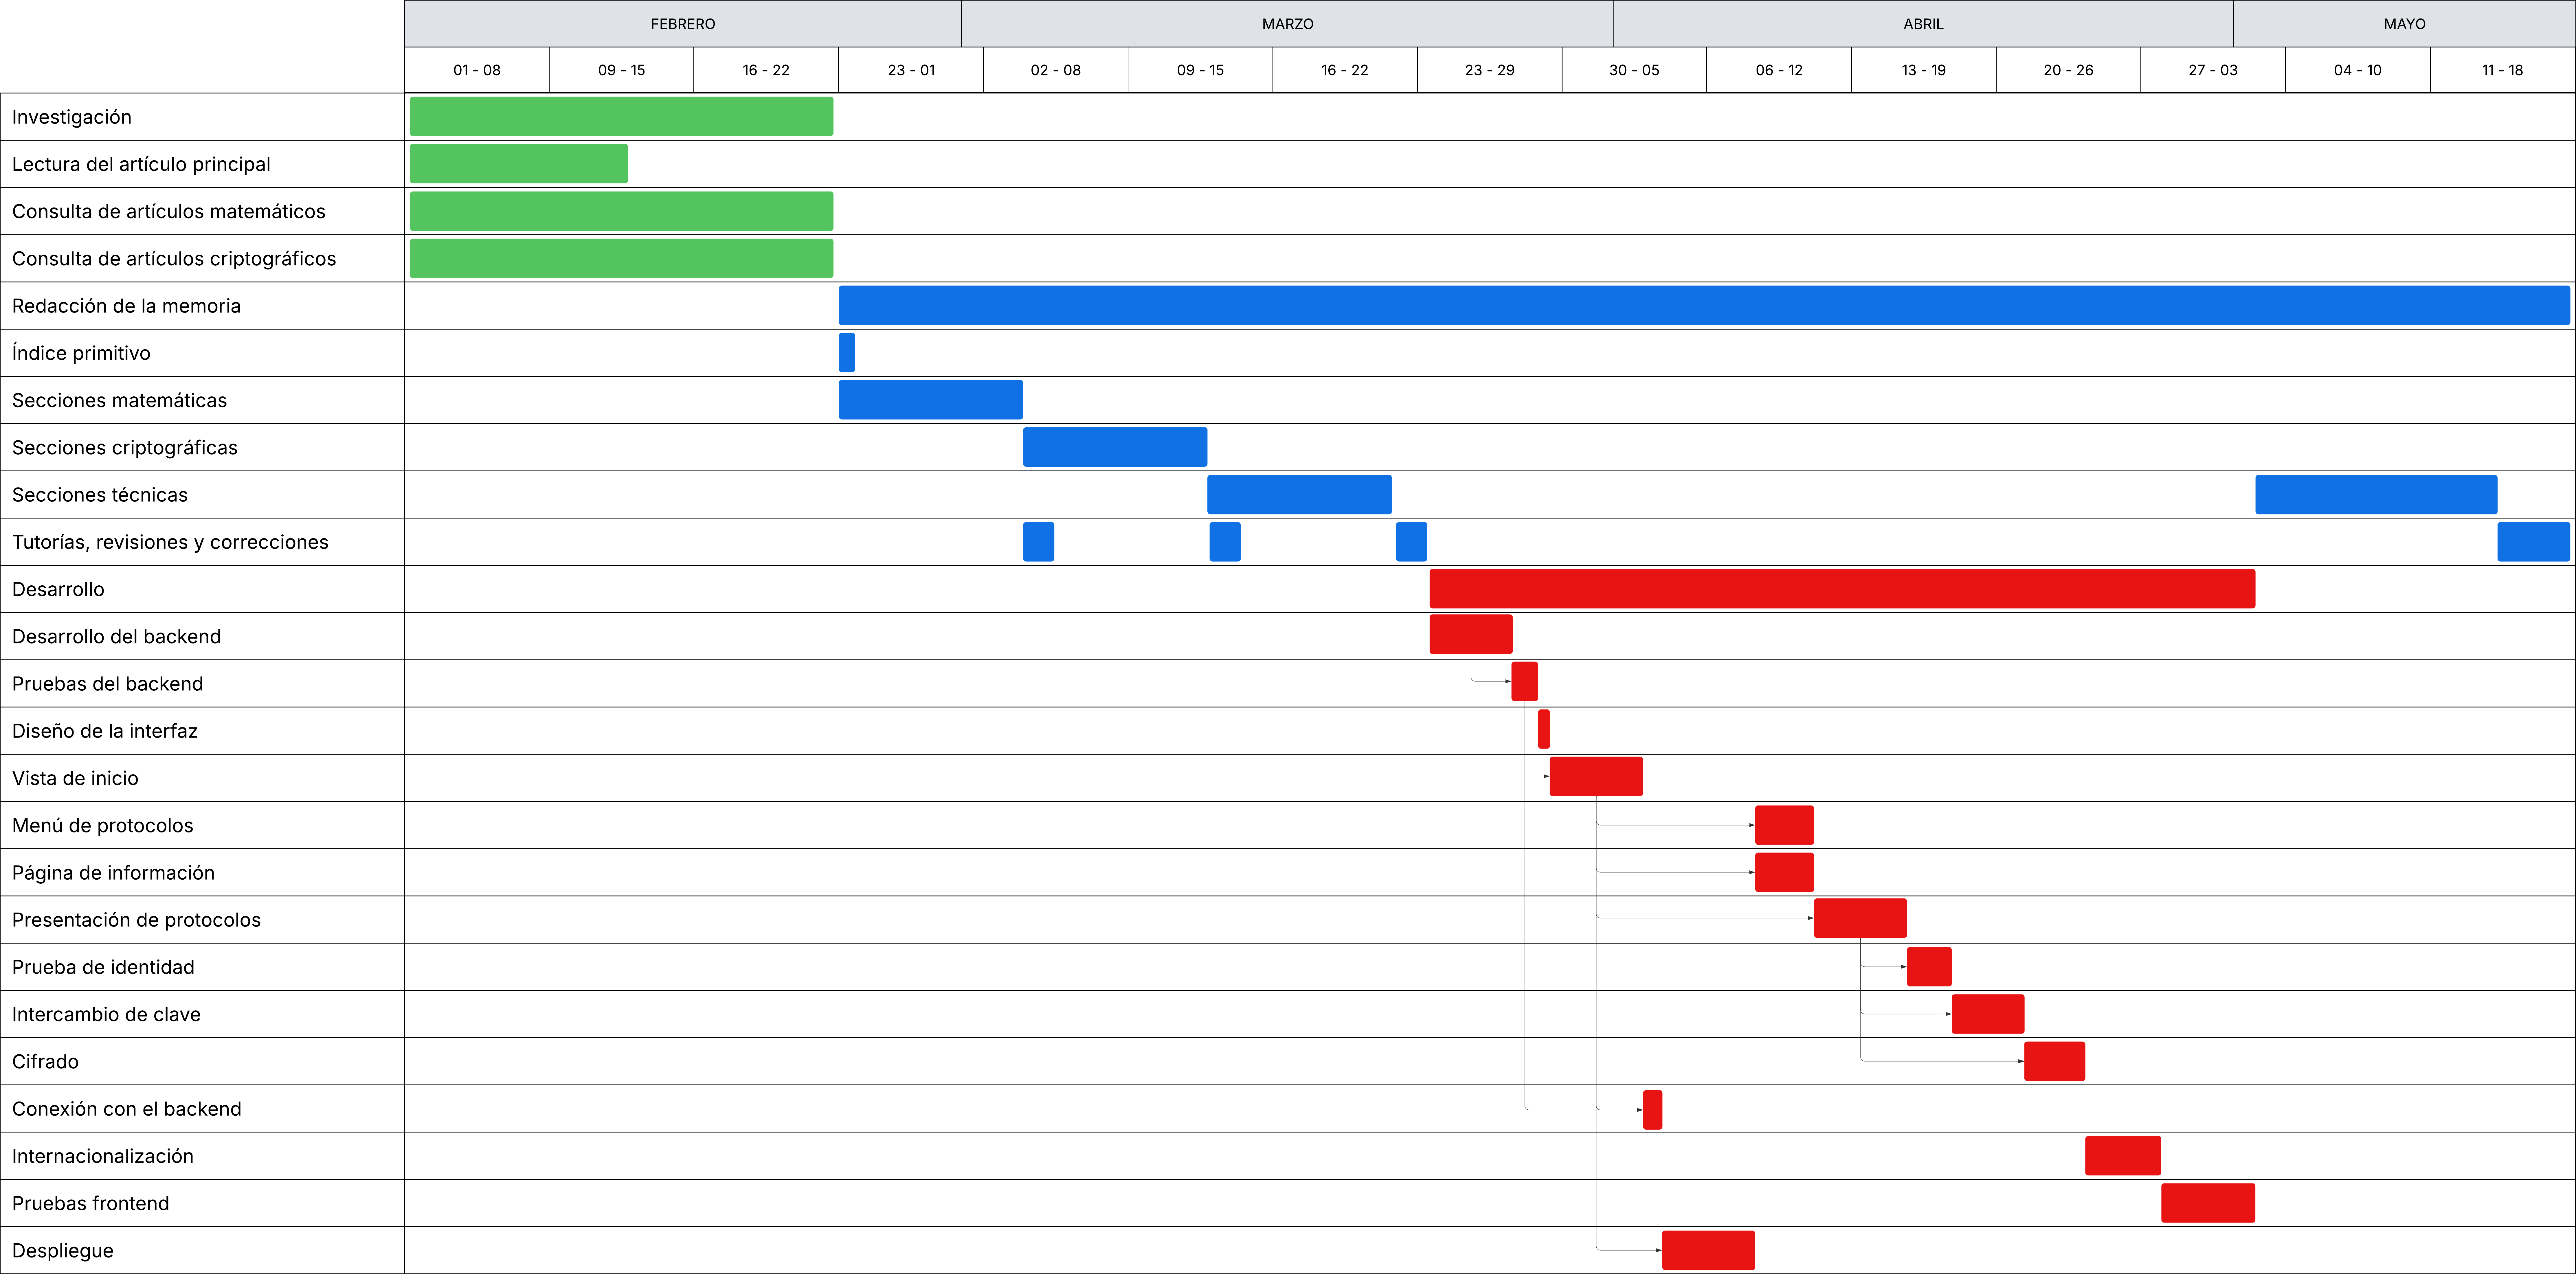
\includegraphics[width=\linewidth]{img/cronograma-original.png}
    \caption{Cronograma original}
    \label{fig:cronograma-original}
\end{figure}
\end{landscape}

\begin{landscape}
\begin{figure}[!ht]
    \centering
    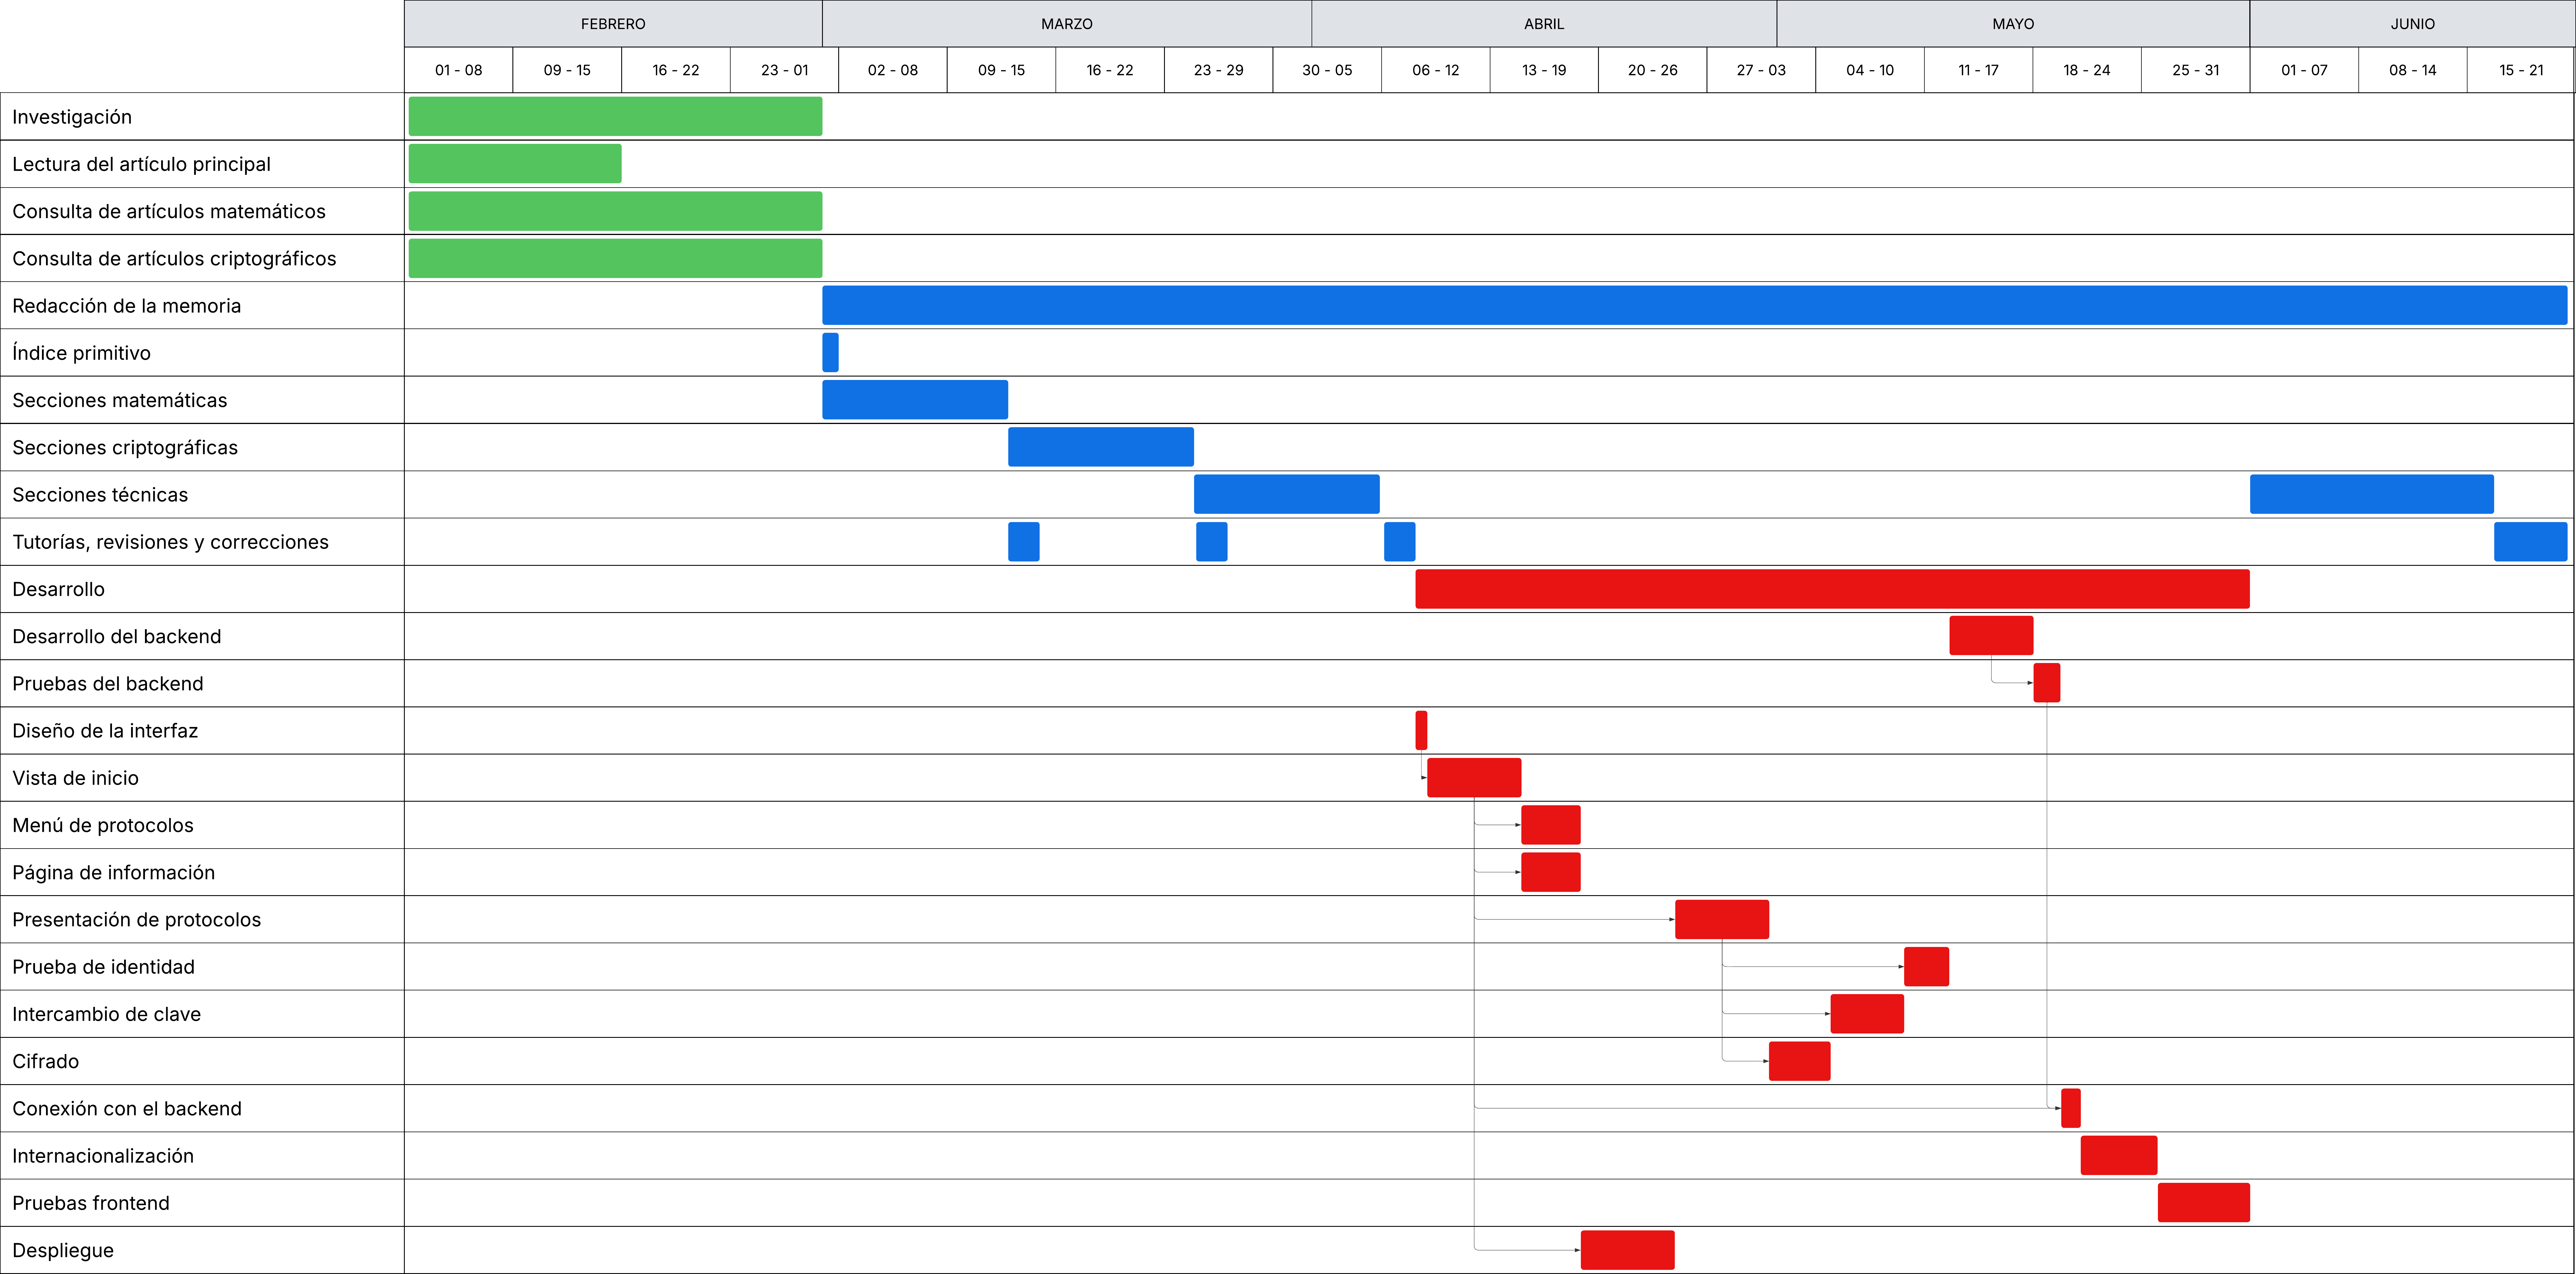
\includegraphics[width=\linewidth]{img/cronograma-real.png}
    \caption{Cronograma real}
    \label{fig:cronograma-real}
\end{figure}
\end{landscape}



\section{Costes}

Para calcular un coste total estimado del proyecto, utilizaremos la fórmula del Total Cost of Ownership o TCO, que contempla tanto gastos de capital como gastos operativos.

Los gastos de capital o CapEx incluyen los gastos materiales como son el ordenador y otros aparatos tecnológicos que se hayan utilizado. Los gastos operativos o OpEx incluyen los costes del personal así como los costes de licencias software que se hayan utilizado.

No se considerarán otros costes relacionados con la electricidad o la conexión a internet al no poder determinar con seguridad su impacto en el desarrollo del proyecto.

Una vez tengamos los costes de capital y operativos calculados, podremos calcular el TCO como

\[ TCO = CapEx + OpEx \]

Sin embargo la estimación no se termina ahí ya que este se considera el coste base del proyecto, hay que tener en cuenta los márgenes de contingencia, el beneficio y el IVA.


\begin{table}[!ht]
    \centering
    \begin{tabular}{ccc}\toprule
         \textbf{Concepto}&  \textbf{Porcentaje}& \textbf{Fórmula}\\\midrule
         Márgenes de contingencia& $10\%$&$0,1 \cdot TCO$\\
         Beneficio& $10\%$&$0,1 \cdot TCO$\\ \hline
         \textbf{Subtotal}& &$0,2 \cdot TCO$\\ \hline
         IVA (21\%)& $21\%$&$0.21 \cdot Subtotal$\\ \hline
         \textbf{Total}&  & $Subtotal + IVA$\\ \bottomrule
    \end{tabular}
    \caption{Coste final una vez calculado el TCO}
    \label{tab:formulas-TCO}
\end{table}

\subsection{Costes de capital}

Como costes de material del proyecto contamos la amortización del ordenador utilizado para el desarrollo: un portátil MSI Prestige 15 A12USCX con un valor de mercado aproximado de 1100€.

Según la Agencia Tributaria, los sistemas informáticos se pueden amortizar con un coeficiente lineal máximo del 26\% \cite{agencia-tributaria-amortizacion}. Considerando un desarrollo aproximado de 5 meses, el coste lo hemos calculado como

\[ \frac{26}{100} \cdot \frac{5}{12} \cdot 1100 = 119,17 €  \]

No vamos a considerar más amortizaciones por motivos similares a el porqué no consideramos el coste de las infraestructuras. Esto junto a que el coste material es el único que vamos a considerar en el CapEx, nos resulta en lo siguiente:

\[ CapEx = 119,17 € \]

\subsection{Costes operativos}

\subsubsection{Gastos de personal}

Para el cálculo de los costes de personal tomamos como referencia el informe de mercado de perfiles informáticos realizado por la Consejería de Agricultura, Pesca y Desarrollo Rural de la Junta de Andalucía \cite{precios}. Dado que se trata de un trabajo fin de grado, consideraremos los perfiles Junior para todos los roles.

A partir del listado de tareas en la sección anterior, haremos la siguiente división de horas que equivaldrá al correspondiente coste.

\begin{table}[!ht]
    \centering
    \begin{tabular}{ccll}\toprule
        \textbf{Rol}& \textbf{Horas}& \textbf{Tarifa (€/h)}&\textbf{Coste}\\\midrule
        Jefe de proyecto& 50& 39,16&1.958\\
        Desarrollador&  121.5& 24,10&2.928,15\\
        Tester de calidad&  20& 23,77&475,4\\ \hline
        \textbf{Total}& 191,5& &5.361,65\\ \bottomrule
    \end{tabular}
    \caption{Coste de personal estimado}
    \label{tab:coste-personal}
\end{table}

\subsubsection{Software y licencias}

Dado que todas las herramientas que hemos utilizado a lo largo del proyecto han sido gratuitas (GitHub, Render, Overleaf) no consideramos los costes. Finalmente, obtenemos los siguientes gastos operativos estimados:

\[ OpEx = 5.361,65 € \]

\subsection{Estimación final}

Una vez calculados el CapEx y el OpEx, podemos calcular el TCO como base de los costes del proyecto.

\[ TCO = CapEx + OpEx = 119,17 + 5.361,65 = 5480,82 \]

Utilizamos la tabla \ref{tab:formulas-TCO} para hacer las estimaciones finales.\footnote{Se ha realizado un redondeo a dos cifras decimales.}

\begin{table}[!ht]
    \centering
    \begin{tabular}{cc}\toprule
        \textbf{Concepto}& \textbf{Coste estimado}\\\midrule
        Márgenes de contingencia&$548,08$\\
        Beneficio&$548,08$\\ \hline
        \textbf{Subtotal}&$6.576,98$\\ \hline
        IVA (21\%)&$1.381,17$\\ \hline
        \textbf{Total}& $7.958,15$\\ \bottomrule
    \end{tabular}
    \caption{Coste final una vez calculado el TCO}
    \label{tab:calculo-TCO}
\end{table}